%% start of file `cv_german.tex', based on `template_en.tex` by Xavier Danaux (xdanaux@gmail.com).
% This work may be distributed and/or modified under the
% conditions of the LaTeX Project Public License version 1.3c,
% available at http://www.latex-project.org/lppl/.
% 
% Thomas Quaritsch <t.quaritsch@student.tugraz.at>

\documentclass[11pt,a4paper]{moderncv}
\usepackage[german]{babel}
\usepackage{moderncv-additions}
\usepackage{pdfpages}
\usepackage{url}

% moderncv themes
\moderncvtheme{casual}   % optional arguments are 'blue' (default), 'orange', 'red', 'green', 'grey' and 'roman' (for roman fonts, instead of sans serif fonts)
%\moderncvtheme[green]{classic}                % idem

% character encoding
\usepackage[utf8]{inputenc}                   % replace by the encoding you are using

% adjust the page margins
\usepackage[scale=0.8]{geometry}
\setlength{\hintscolumnwidth}{3cm}			  % if you want to change the width of the column with the dates
%\AtBeginDocument{\setlength{\maketitlenamewidth}{6cm}}  % only for the classic theme, if you want to change the width of your name placeholder (to leave more space for your address details


\AtBeginDocument{\recomputelengths}           % required when changes are made to page layout lengths

% personal data
\firstname{Simon}
\familyname{Szustkowski}
%\title{Resumé title (optional)}               % optional, remove the line if not wanted
\address{Marsbruchstraße 117}{44287 Dortmund}        % optional, remove the line if not wanted
\mobile{+49 176 24692840}                     % optional, remove the line if not wanted
\phone{+49 231 3306614}                      % optional, remove the line if not wanted
%\fax{fax (optional)}                          % optional, remove the line if not wanted
\email{mail@simonszu.de}                      % optional, remove the line if not wanted
%\extrainfo{additional information (optional)} % optional, remove the line if not wanted
\photo[64pt]{picture}                          % '64pt' is the height the picture must be resized to and 'picture' is the name of the picture file; optional, remove the line if not wanted
%\quote{``Das ist ein toller Frusterspruch\\ von Friede Frusterfrau.'' -- Friede Frusterfrau}                 % optional, remove the line if not wanted

%\nopagenumbers{}                             % uncomment to suppress automatic page numbering for CVs longer than one page


%----------------------------------------------------------------------------------
%            content
%----------------------------------------------------------------------------------

\begin{document}

% color redefinitions must be after \begin{document}!
\definecolor{firstnamecolor}{RGB}{125,85,85}
\definecolor{familynamecolor}{RGB}{138,74,57}
\definecolor{quotecolor}{RGB}{125,85,85}
\definecolor{addresscolor}{RGB}{125,85,85}
\definecolor{sectionrectanglecolor}{RGB}{138,74,57}
\definecolor{sectiontitlecolor}{RGB}{138,74,57}
\definecolor{subsectioncolor}{RGB}{125,85,85}
\definecolor{footersymbolcolor}{RGB}{125,85,85}	

\makeatletter

\pagestyle{empty}
\chapter*{Curriculum }{Vitae}

\vspace*{50mm}
\begin{minipage}{\textwidth}
	\vspace*{3mm}
	\familynamestyle{\@firstname}~~\firstnamestyle{\@familyname} 	
	\hspace*{5mm}{{\color{firstnamecolor}\includegraphics[width=64pt]{picture}}}\\[3mm]
	\@addressstreet, \@addresscity ~~~ \mobilesymbol~\@mobile ~~~ \emailsymbol~\@email
\end{minipage}
\begin{minipage}{70pt}
	
\end{minipage}

\vfill

\begin{minipage}{1.0\textwidth}
	\section{Inhalt}
	\tableofcontents
\end{minipage}

\newpage
\pagestyle{fancy}
%\chapter{Curriculum}{~Vit\ae}
\chapter{Curriculum Vitae}{}
\makequote

\section{Persönliche Daten}
%%%%%%%%%%%%%%%%%%%%%%%%%%%%%%%%%%%%%%%%%%%%%%%%%%%%%%%%%%%%%%%%%%%%
\cvline{Name}{\@firstname~\@familyname}
\cvline{Anschrift}{\@addressstreet, \@addresscity}
\cvline{Telefon}{\@mobile}
\cvline{E-Mail}{\@email}
\cvline{Geburtsdatum}{11. Februar 1988 in Münster}
\cvline{Staatsbürgerschaft}{Deutschland / Schweiz}
%\cvline{Familienstand}{ledig}
%\cvline{Präsenzdienst}{abgeleistet}
\cvline{Führerschein}{B}
\makeatother 

%\cventry{year--year}{Degree}{Institution}{City}{\textit{Grade}}{Description}  % arguments 3 to 6 are optional

\section{Ausbildung} 
%%%%%%%%%%%%%%%%%%%%%%%%%%%%%%%%%%%%%%%%%%%%%%%%%%%%%%%%%%%%%%%%%%%%

\cventry{10/2009 -- 04/2018}{Bachelor of Science}{Technische Universität}{Dortmund}{\textit{Informatik}}{Nebenfach: Maschinenbau}  % arguments 3 to 6 are optional

\cventry{09/2006 -- 06/2009}{Mechatroniker (IHK)}{Miele \& Cie. KG}{Bielefeld}{}{Zusätzlich: Elektrofachkraft} 

\section{Berufserfahrung} 
%%%%%%%%%%%%%%%%%%%%%%%%%%%%%%%%%%%%%%%%%%%%%%%%%%%%%%%%%%%%%%%%%%%%

\cventry{01/2021 -- heute}{Senior Consultant}{VIADA GmbH \& Co. KG}{Dortmund}{}{Cloud-Infrastruktur und DevOps Engineering mit Schwerpunkt Red Hat OpenShift und Ansible, mit Team-Lead-Aufgaben im Projektteam}
\cventry{05/2018 -- 01/2021}{Consultant}{VIADA GmbH \& Co. KG}{Dortmund}{}{Cloud-Infrastruktur und DevOps Engineering mit Schwerpunkt Red Hat OpenShift und Ansible}
\cventry{12/2012 -- 04/2018}{Administrator des Wide Area Networks}{ECOFIS GmbH}{Dortmund}{}{}
\cventry{10/2010 -- 11/2012}{First Level Support}{Sozialforschungsstelle der Technischen Universität}{Dortmund}{}{}
\cventry{09/2006 -- 06/2009}{Auszubildender zum Mechatroniker (IHK)}{Miele \& Cie. KG}{Bielefeld}{}{}

\section{Projektrückblick}
\cventry{04/2023 -- heute}{Aufbau und Betrieb von containerbasierter Edge-Infrastruktur}{Mittelständisches Unternehmen für Software in der industriellen Fertigung}{Limburg a.d. Lahn}{}{Erarbeiten und Umsetzen eines Konzeptes zur automatischen Provisionierung und Betrieb von OpenShift-Instanzen, die als Edge-Lösung bei Endkunden in der Fertigung Software zum Manufacturing Operation Management hosten sollen.}
\cventry{12/2022 -- 03/2023}{Infrastruktursetup Security-Gateway}{Weltweit tätiger IT- und Telekommunikationsdienstleister}{Wolfsburg}{}{Setup und Inbetriebnahme einer Cloud-Infrastruktur zum Betrieb eines Security-Gateways für eine eID-Anwendung nach Vorgaben der Bundesdruckerei als verantwortlicher Engineer.}
\cventry{04/2022 --11/2022}{Infrastruktursetup Logistikprojekt}{Weltweit tätiger IT- und Telekommunikationsdienstleister}{Wolfsburg}{}{Setup und Inbetriebnahme einer Cloud-Infrastruktur zum Betrieb einer Anwendung mit dem Ziel, Lieferscheine digital zu verwalten. Das System konnte nach Vorgaben der GS1 Germany zeitgenau in Betrieb genommen werden und hat während meines Mitwirkens im Projekt nach einer PoC-Phase die ersten Kunden gewinnen können.}
\cventry{01/2022 -- 03/2022}{Automatsierung VoIP}{Weltweit tätiger IT- und Telekommunikationsdienstleister}{Wolfsburg}{}{Automatisierung der Einrichtung eines auf Jitsi basierenden VoIP-Stacks aus 5-8 VMs für einen Endkunden aus dem Gesundheitswesen mit Ansible als verantwortlicher Engineer. \\Erreicht wurde eine Verkürzung des Time-to-market bei Neukunden von ca 10 Tagen auf einen Tag.}
\cventry{10/2021 -- 12/2021}{Monitoring Anwendungsbetrieb}{Automobilindustrieunternehmen}{Sindelfingen}{}{Konzeptionierung und Umsetzung einer auf dem Prometheus-Stack basierenden Monitoringlösung im Rahmen einer Cloud-Migration von Bare-Metal auf Microsoft Azure. \\Hierdurch wurde dem Kunden, der zuvor nur reaktives Monitoring mit Icinga verwendet hat, ermöglicht proaktiv auf sich abzeichnende Trends der einzelnen Metriken zu reagieren.}
\cventry{08/2021 -- 09/2021}{Consulting Shopware as a Service}{Weltweit tätiger IT- und Telekommunikationsdienstleister}{Wolfsburg}{}{Leitender Infrastruktur-Architekt zur Bereitstellung einer Shopware-Plattform als SaaS-Lösung auf Basis der Open Telekom Cloud. \\ Technische Migration einer bestehenden Shopware-Plattform auf cloud-native Infrastruktur bei gleichzeitiger Konsolidierung des Betriebsteams auf Grundlage der DSGVO.}
\cventry{01/2020 -- 07/2021}{OpenShift Architekturoptimierung}{Automobilindustrieunternehmen}{München}{}{Begleitung des Endkundens aus der Automobilindustrie im Hinblick auf eine effiziente agile Transformation des Plattform-Betriebsteams mit dem Schwerpunkt GitOps. \\In einem Engineering-Team wurde durch Erarbeitung, Etablierung und kontinuierliche Verbesserung agiler Prozesse das Daily Business von reinem Problem Engineering zu Feature Engineering entwickelt, weswegen im Laufe des Projektes der Wunsch nach besserer Nachverfolgbarkeit und Versionierung der Feature-Deployments aufkam, welcher mit der Einführung von ArgoCD in den Prozessen des internationalen Betriebsteams erfüllt wurde.}
\cventry{01/2019 -- 12/2019}{Einführung OpenShift}{Genossenschaftliche Zentralbank}{Frankfurt a.M}{}{Technische Einführung von Red Hat OpenShift mit besonderem Fokus auf kundenspezifische Anforderungen bezüglich Security und Compliance nach BaFin-Standard. \\ Als Plattformbetriebsteam von insgesamt vier OpenShift-Clustern wurden Wege erarbeitet, die Vorgaben der BaFin umzusetzen, u.a. Hardening der Cluster, Einrichtung georedundanter Backups, das Sammeln und Auswerten von Logfiles mit einer Retention von 10 Jahren, sowie automatisierter Container- und Image-Security-Checks.}
\cventry{07/2018 -- 12/2018}{Installation und Konfiguration von AppAgile auf der Open Telekom Cloud}{Europaweit tätiges Logistikunternehmen}{Hamburg}{}{Enablement des Kunden zum Entwickeln containerbasierter Anwendungen, Einführung eines Backup-Prozesses mit Hilfe von restic und der Open Telekom Cloud}

\section{Zertifizierungen}
\cventry{06/2024}{Fachkraft für agile Führung (IHK)}{thekey.career}{}{Zertifikats-ID: ac-2024-be5250}{}
\cventry{06/2021}{Specialist in Containers and Kubernetes}{Red Hat}{}{Zertifikats-ID: 200-059-038}{}
\cventry{03/2020}{Specialist in Ansible Automation}{Red Hat}{}{Zertifikats-ID: 200-059-038}{}
\cventry{07/2013}{IPv6 Sage}{Hurricane Electric}{}{}{}
\cventry{07/2009}{Elektrofachkraft}{Industrie- und Handelskammer}{Ostwestfalen zu Bielefeld}{}{}
\cventry{01/2007}{Funkamateur Klasse E}{Bundesnetzagentur}{Münster}{}{}

\section{Sprachen} 
%%%%%%%%%%%%%%%%%%%%%%%%%%%%%%%%%%%%%%%%%%%%%%%%%%%%%%%%%%%%%%%%%%%%

\cvline{Deutsch}{Muttersprache}{}
\cvline{Englisch}{fließend in Wort und Schrift}
\cvline{Französisch}{Grundkenntnisse}
\cvline{Dänisch}{Grundkenntnisse}
\cvline{Niederländisch}{Grundkenntnisse}


\section{Auszeichnungen} 
%%%%%%%%%%%%%%%%%%%%%%%%%%%%%%%%%%%%%%%%%%%%%%%%%%%%%%%%%%%%%%%%%%%%
\cvline{01/2022}{Viada Innovation Award 2022}
\cvline{01/2019}{Viada Subject Matter Expert in IT Automation and Management}
\cvline{01/2019}{Viada Subject Matter Expert in Hybrid Cloud Infrastructure Administration}

%\cvline{xx/xxxx}{Musterpreis}


\section{Außerberufliche Tätigkeiten} 
%%%%%%%%%%%%%%%%%%%%%%%%%%%%%%%%%%%%%%%%%%%%%%%%%%%%%%%%%%%%%%%%%%%%

\cvline{Chaostreff Dortmund e.V.}{Mithilfe auf und Besuch von Events im Umfeld des Chaos Computer Clubs} 
\cvline{Technisches Hilfswerk OV Unna-Schwerte}{Technischer Helfer}
\cvline{Service für Veranstaltungstechnik Matthias van der Wal}{Veranstaltungstechnik der Haupt-Bühnen diverser Conventions für Anime, Manga und Nerd-Kultur als ehrenamtlicher Helfer}

\section{Interessen}
%%%%%%%%%%%%%%%%%%%%%%%%%%%%%%%%%%%%%%%%%%%%%%%%%%%%%%%%%%%%%%%%%%%%

\cvline{Amateurfunk}{Betrieb einer Funkstation im Amateurfunkdienst (Klasse E)}
\cvline{Fotografie}{Architektur- und Landschaftsfotografie}
\cvline{Making}{Elektro- und Programmierprojekte im Umfeld der Maker- und OpenSource-Szene}

\section{Profile}
\cvline{GitHub}{\url{https://github.com/simonszu}}
\cvline{Thingiverse}{\url{https://www.thingiverse.com/ttk_/designs}}
\cvline{Docker Hub}{\url{https://hub.docker.com/u/simonszu}}
\cvline{LinkedIn}{\url{https://www.linkedin.com/in/simonszu/}}
\cvline{Xing}{\url{https://www.xing.com/profile/Simon_Szustkowski}}

%\section{Publikationen} 
%%%%%%%%%%%%%%%%%%%%%%%%%%%%%%%%%%%%%%%%%%%%%%%%%%%%%%%%%%%%%%%%%%%%

%\subsection{Konferenzen und Workshops}

%\cvline{mm/jjjj}{Autor 1 und Autor 2. \textbf{Mustertitel: Unser tolles Paper.} In \textit{Proceedings of the First Muster Workshop 1970}, Musterstadt, Musterland, YYYY.}

% \newpage

%\subsection{Technical Reports}

%\cvline{....}{....}

%\cvline{....}{alternativ kann man auch BibTex verwenden:}

%\renewcommand*{\refname}{Abschlussarbeiten}
%\nocite{*}
%\bibliographystyle{cv}
%\bibliography{publications}       % 'publications' is the name of a BibTeX file


%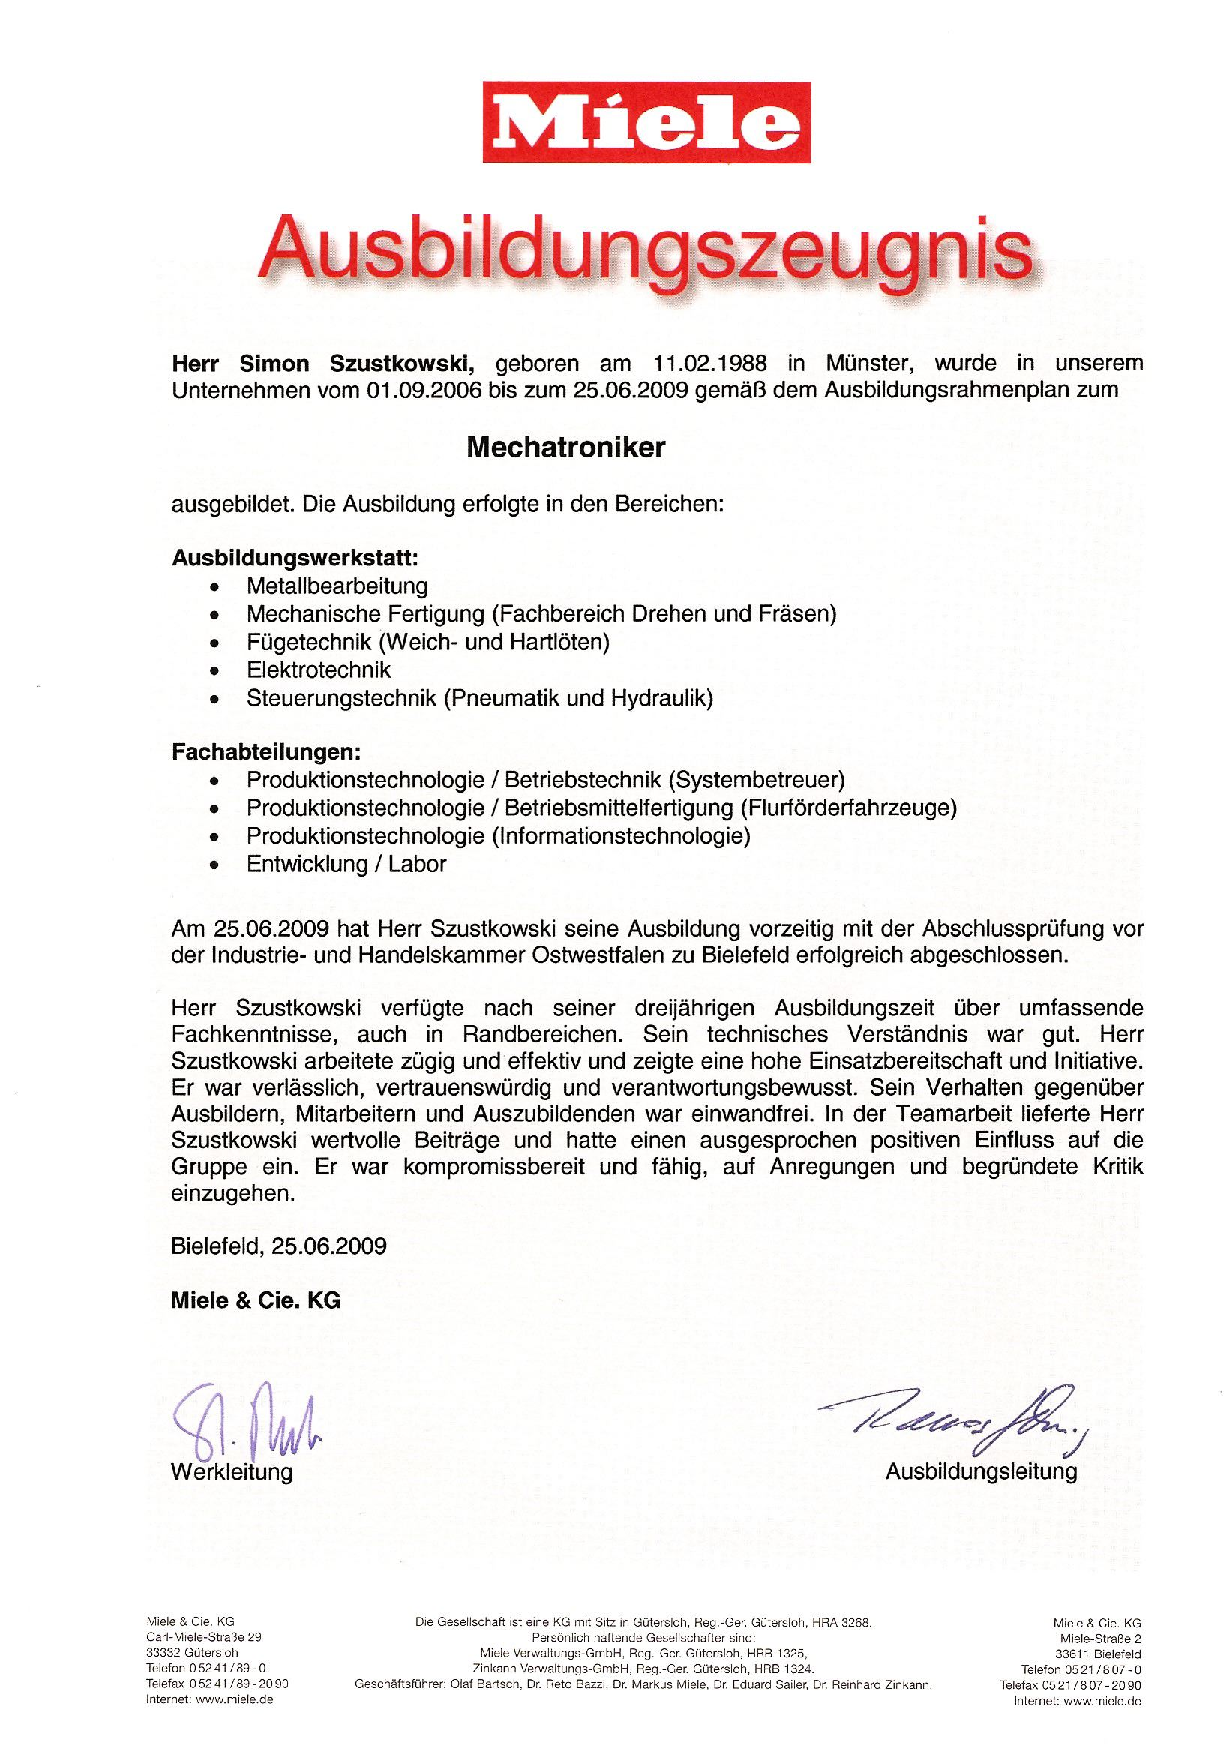
\includepdf[pages=1,addtotoc={
%	4, chapter, 1, Arbeitszeugnis Miele \& Cie. KG, az-miele
%	}]{azmiele.pdf}
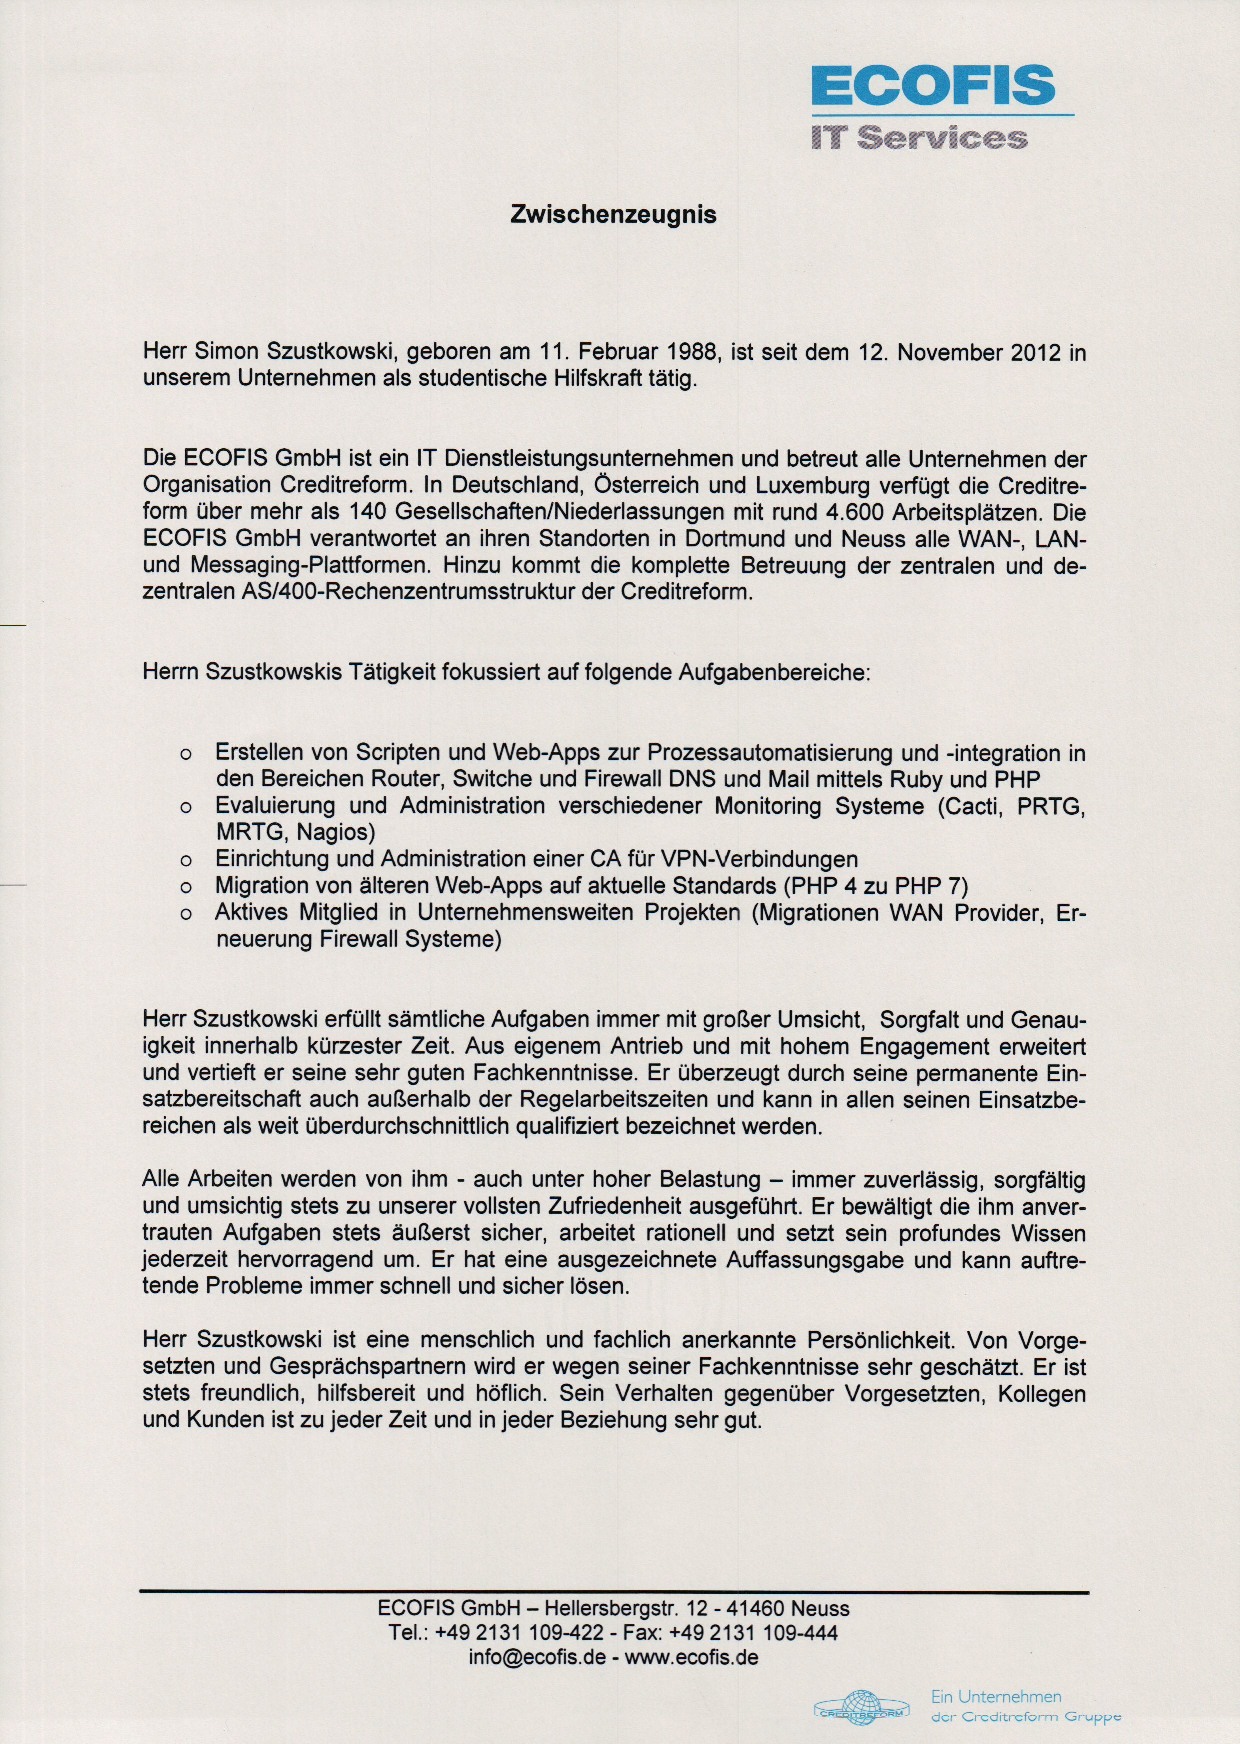
\includepdf[pages=1-,addtotoc={1, section, 1, Arbeitszeugnis ECOFIS GmbH, azecofis} ]{./Arbeitszeugnisse/ECOFIS.pdf}
%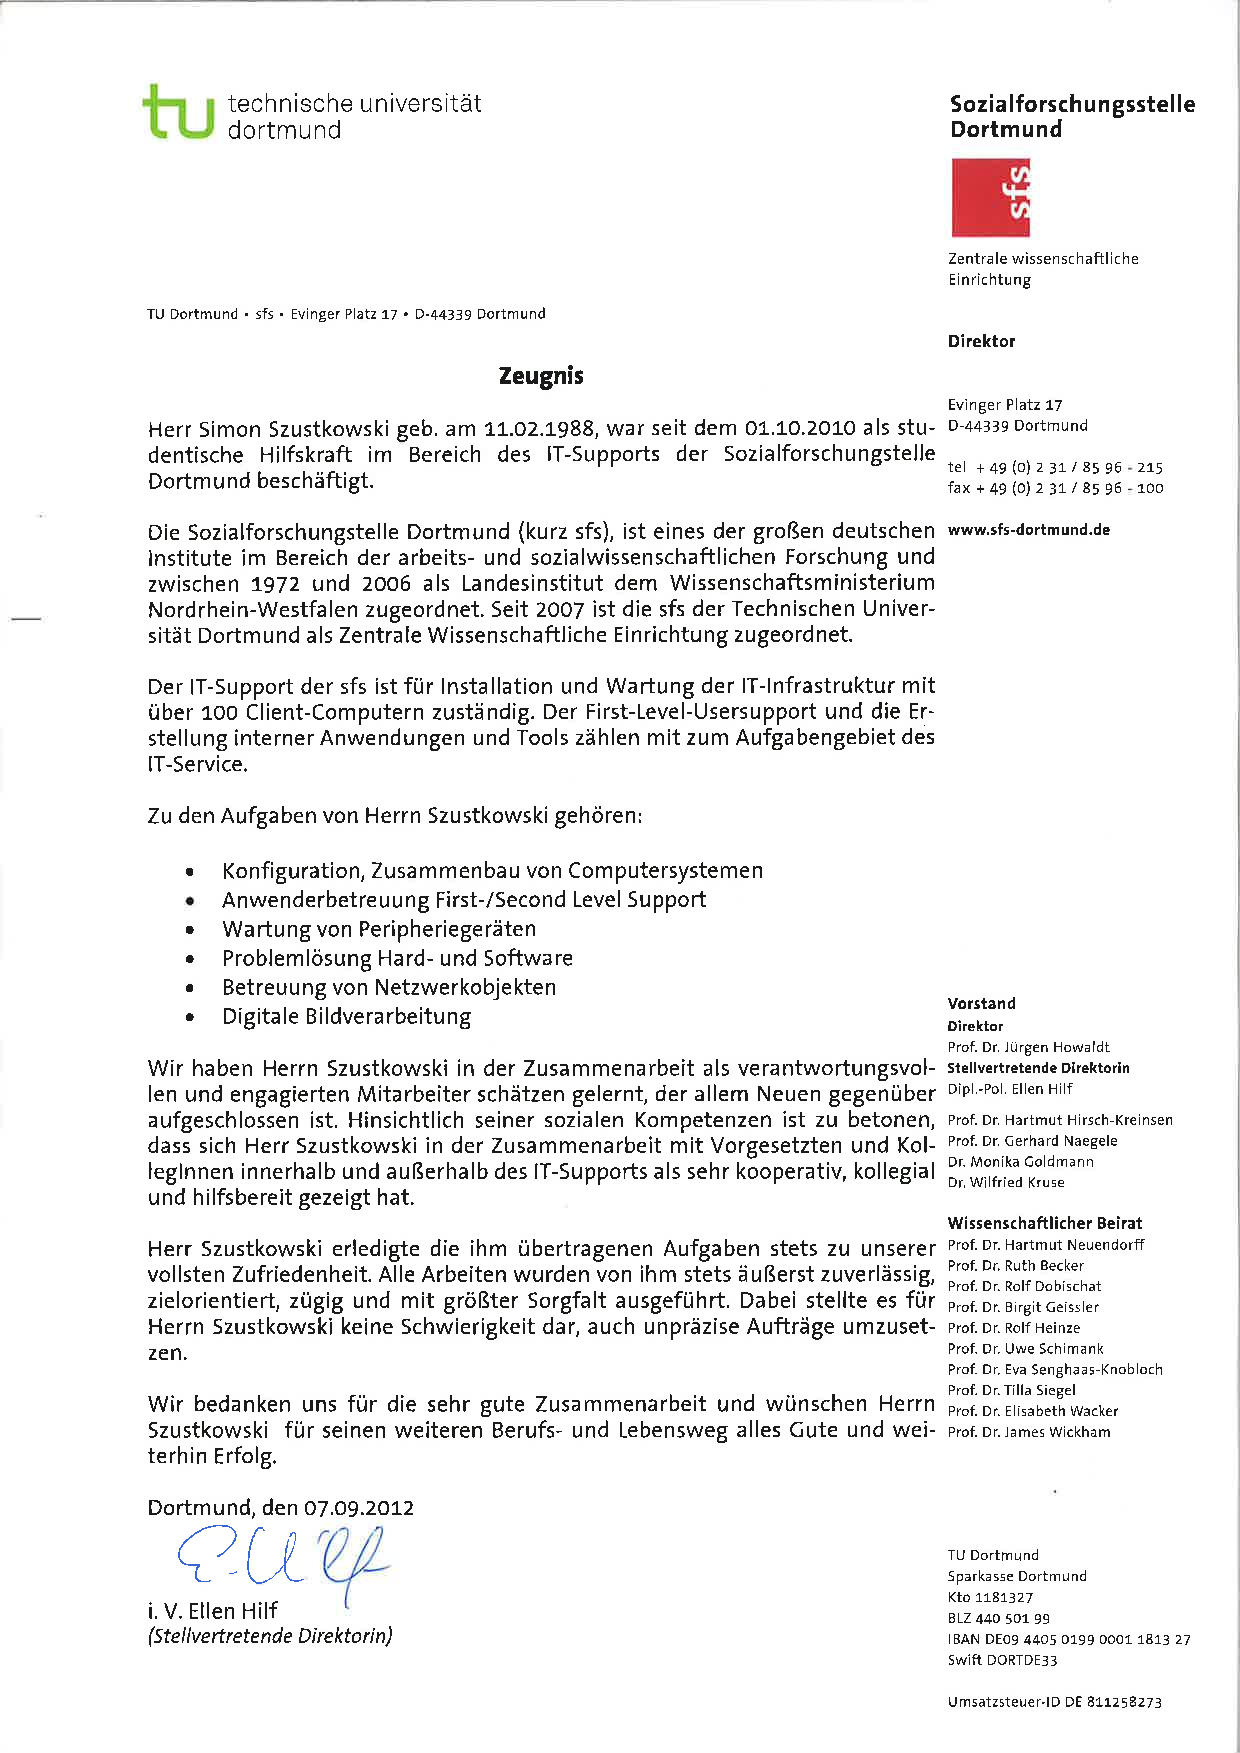
\includepdf[pages=1,addtotoc={1, section, 1, Arbeitszeugnis Sozialforschungsstelle Dortmund, azsfs} ]{./Arbeitszeugnisse/SFS.pdf}
%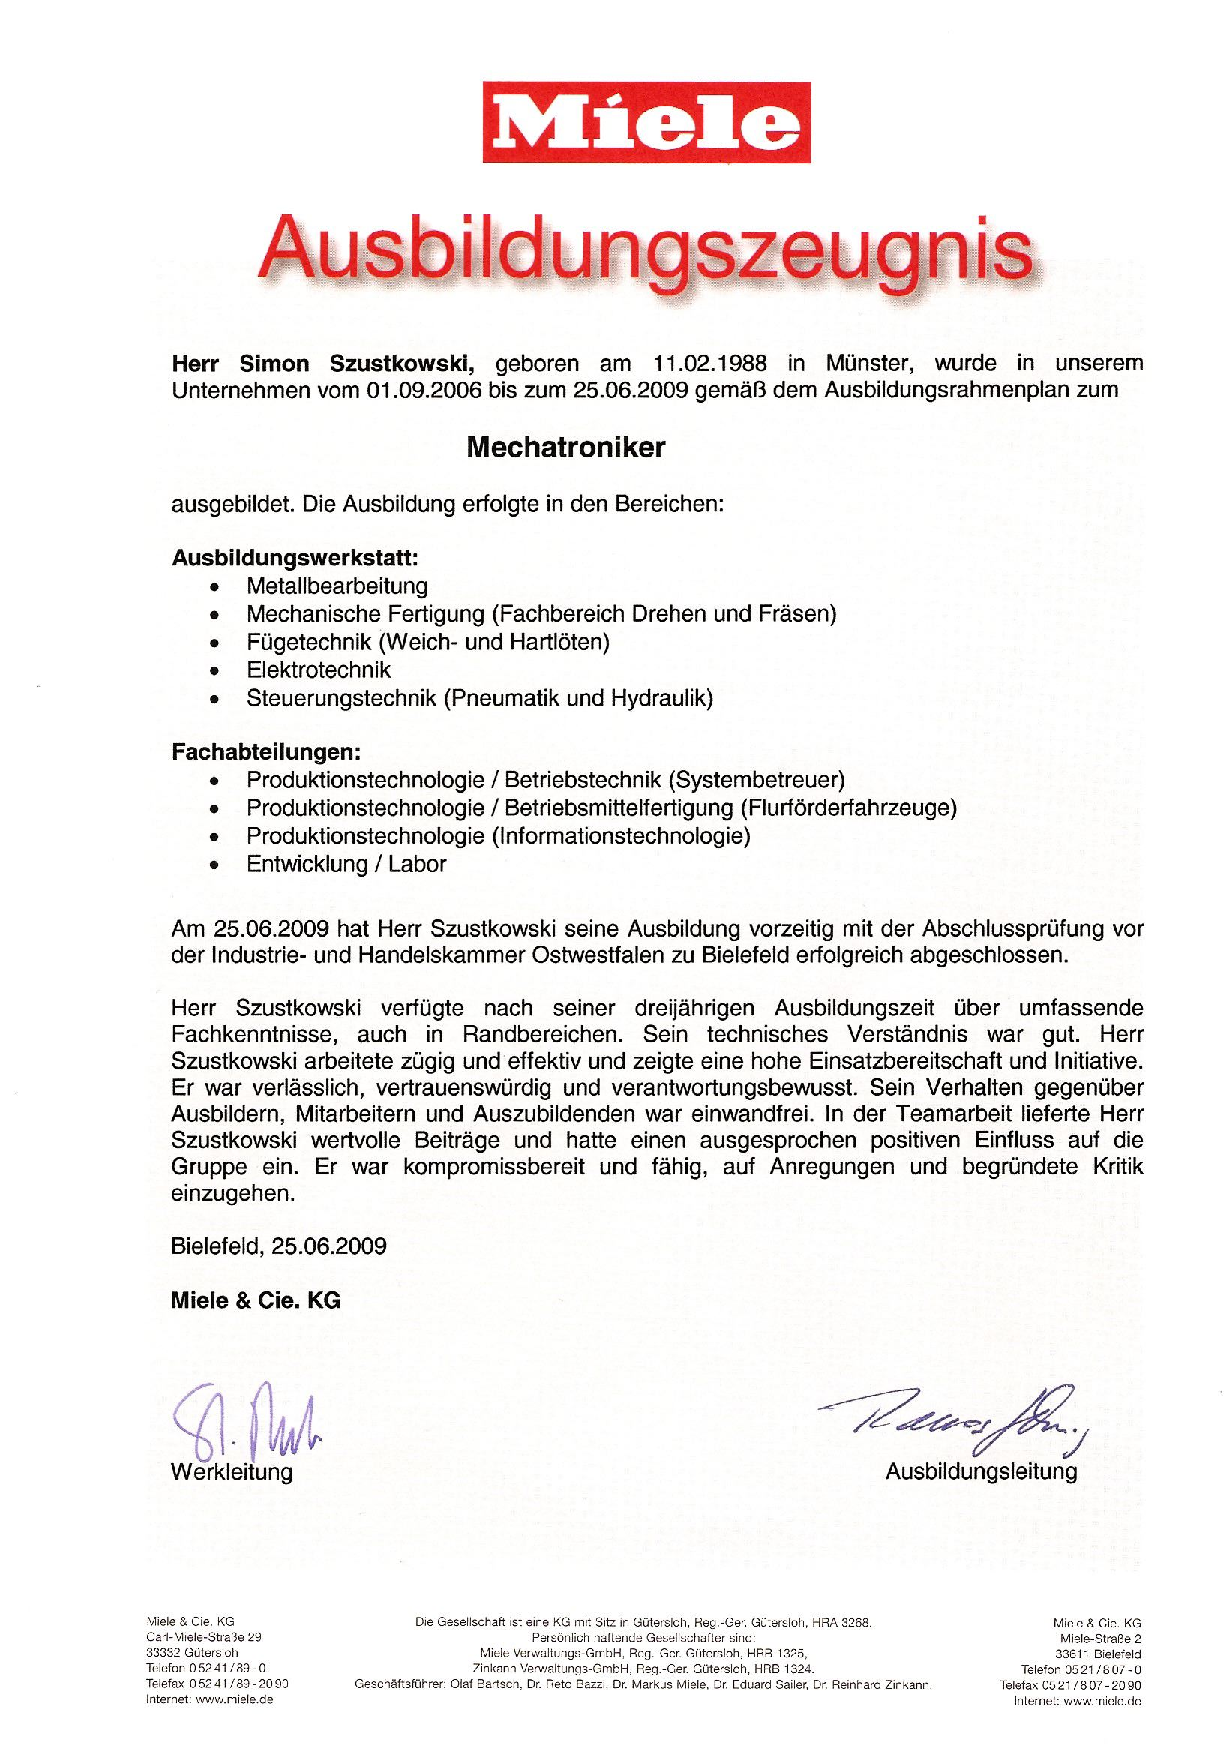
\includepdf[pages=1,addtotoc={1, section, 1, Arbeitszeugnis Miele \& Cie. KG, azmiele} ]{./Arbeitszeugnisse/Miele.pdf}


%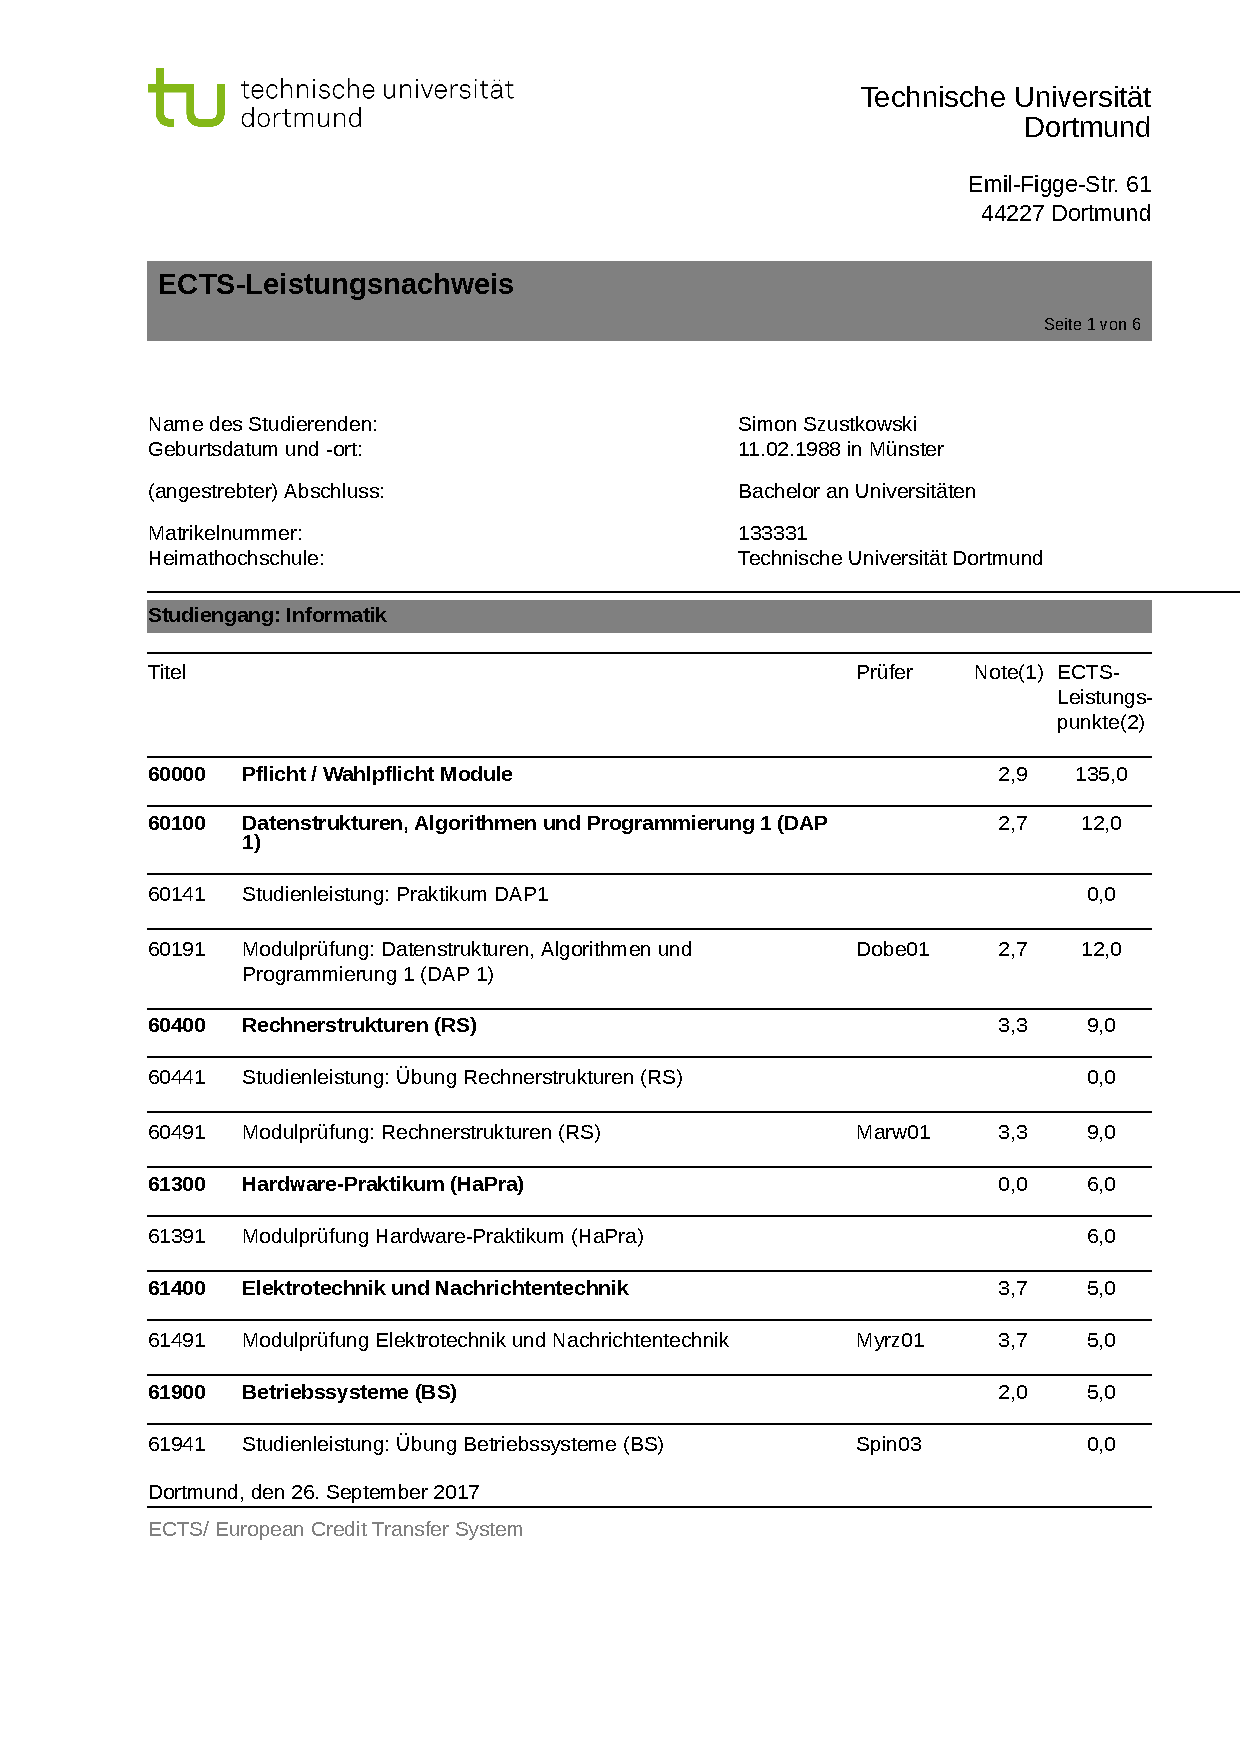
\includepdf[pages=1-,addtotoc={1, section, 1, Notenspiegel, notenspiegel} ]{notenspiegel.pdf}

%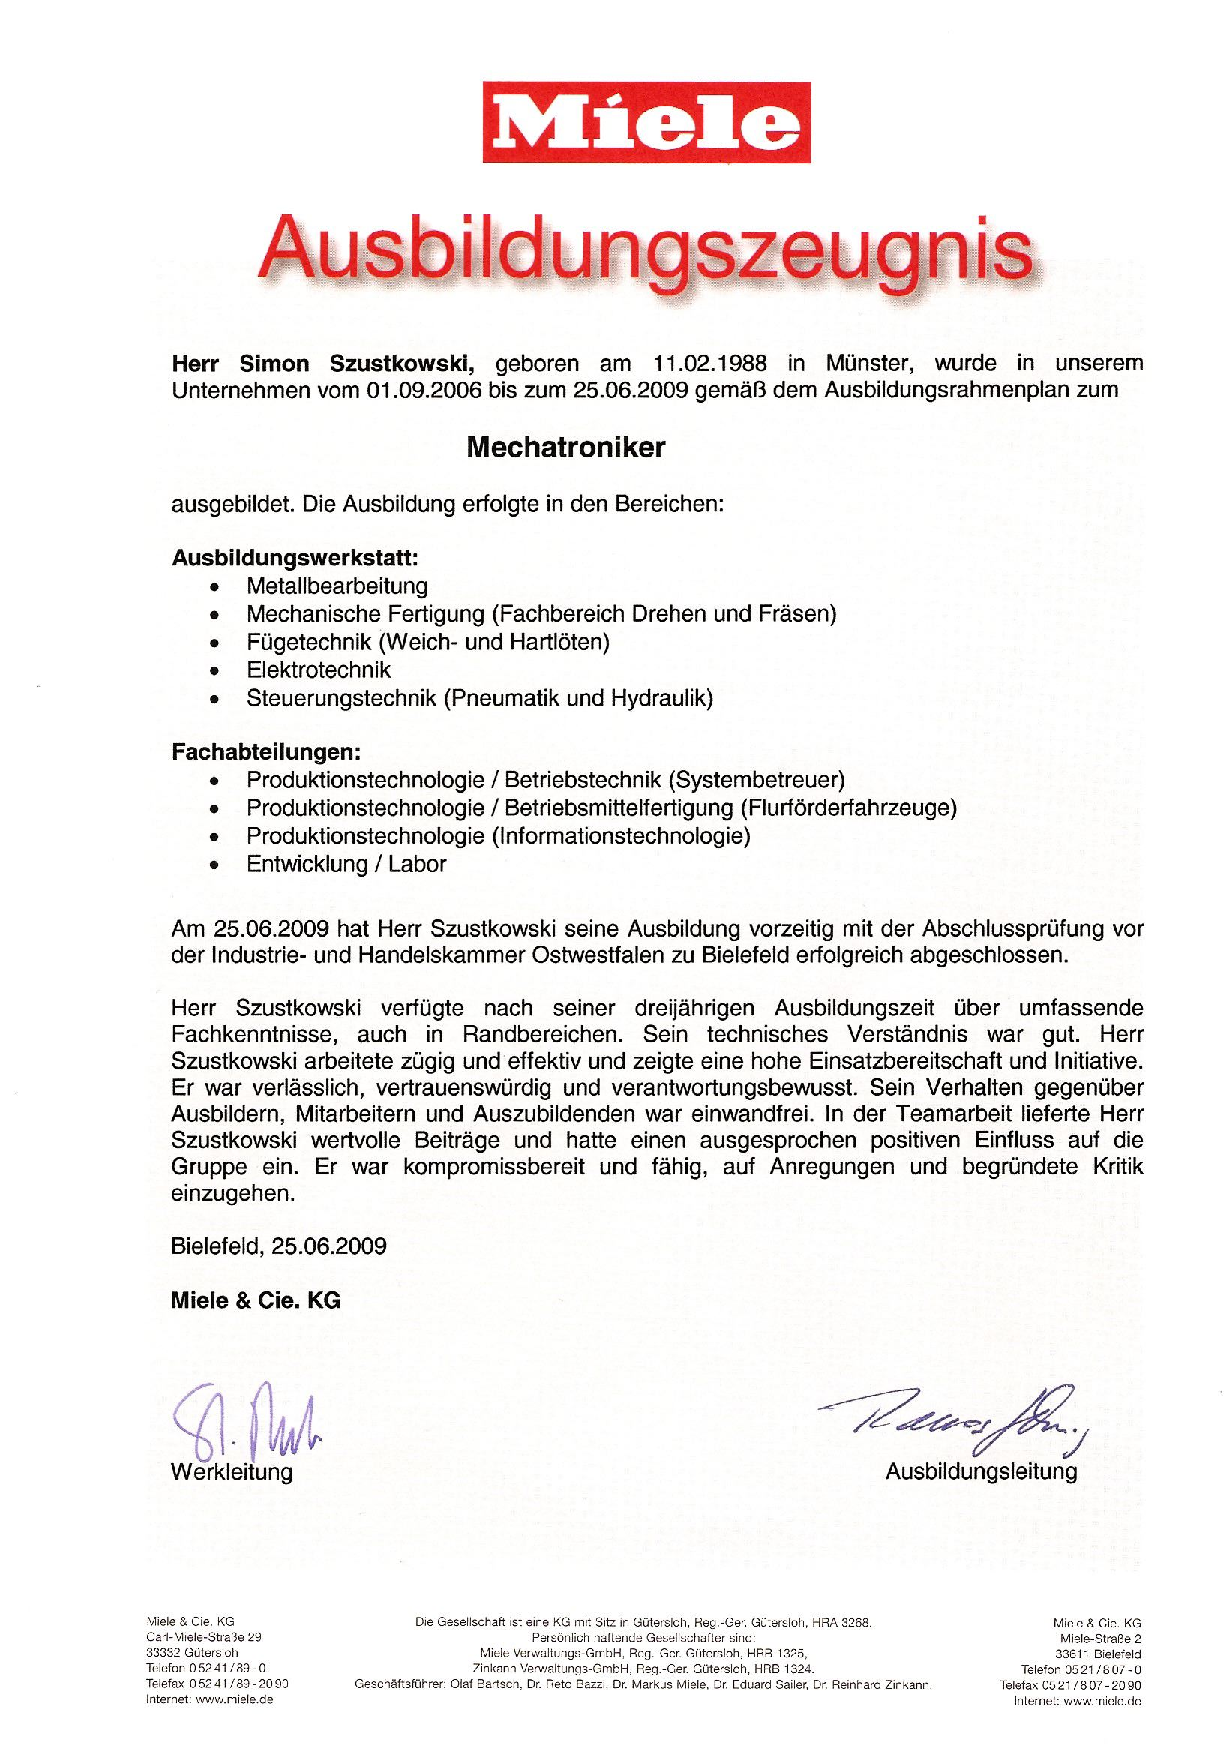
\includepdf[pages=1-,pagecommand={\chapter{Arbeitszeugnis Miele \& Cie. KG}}]{azmiele.pdf}
%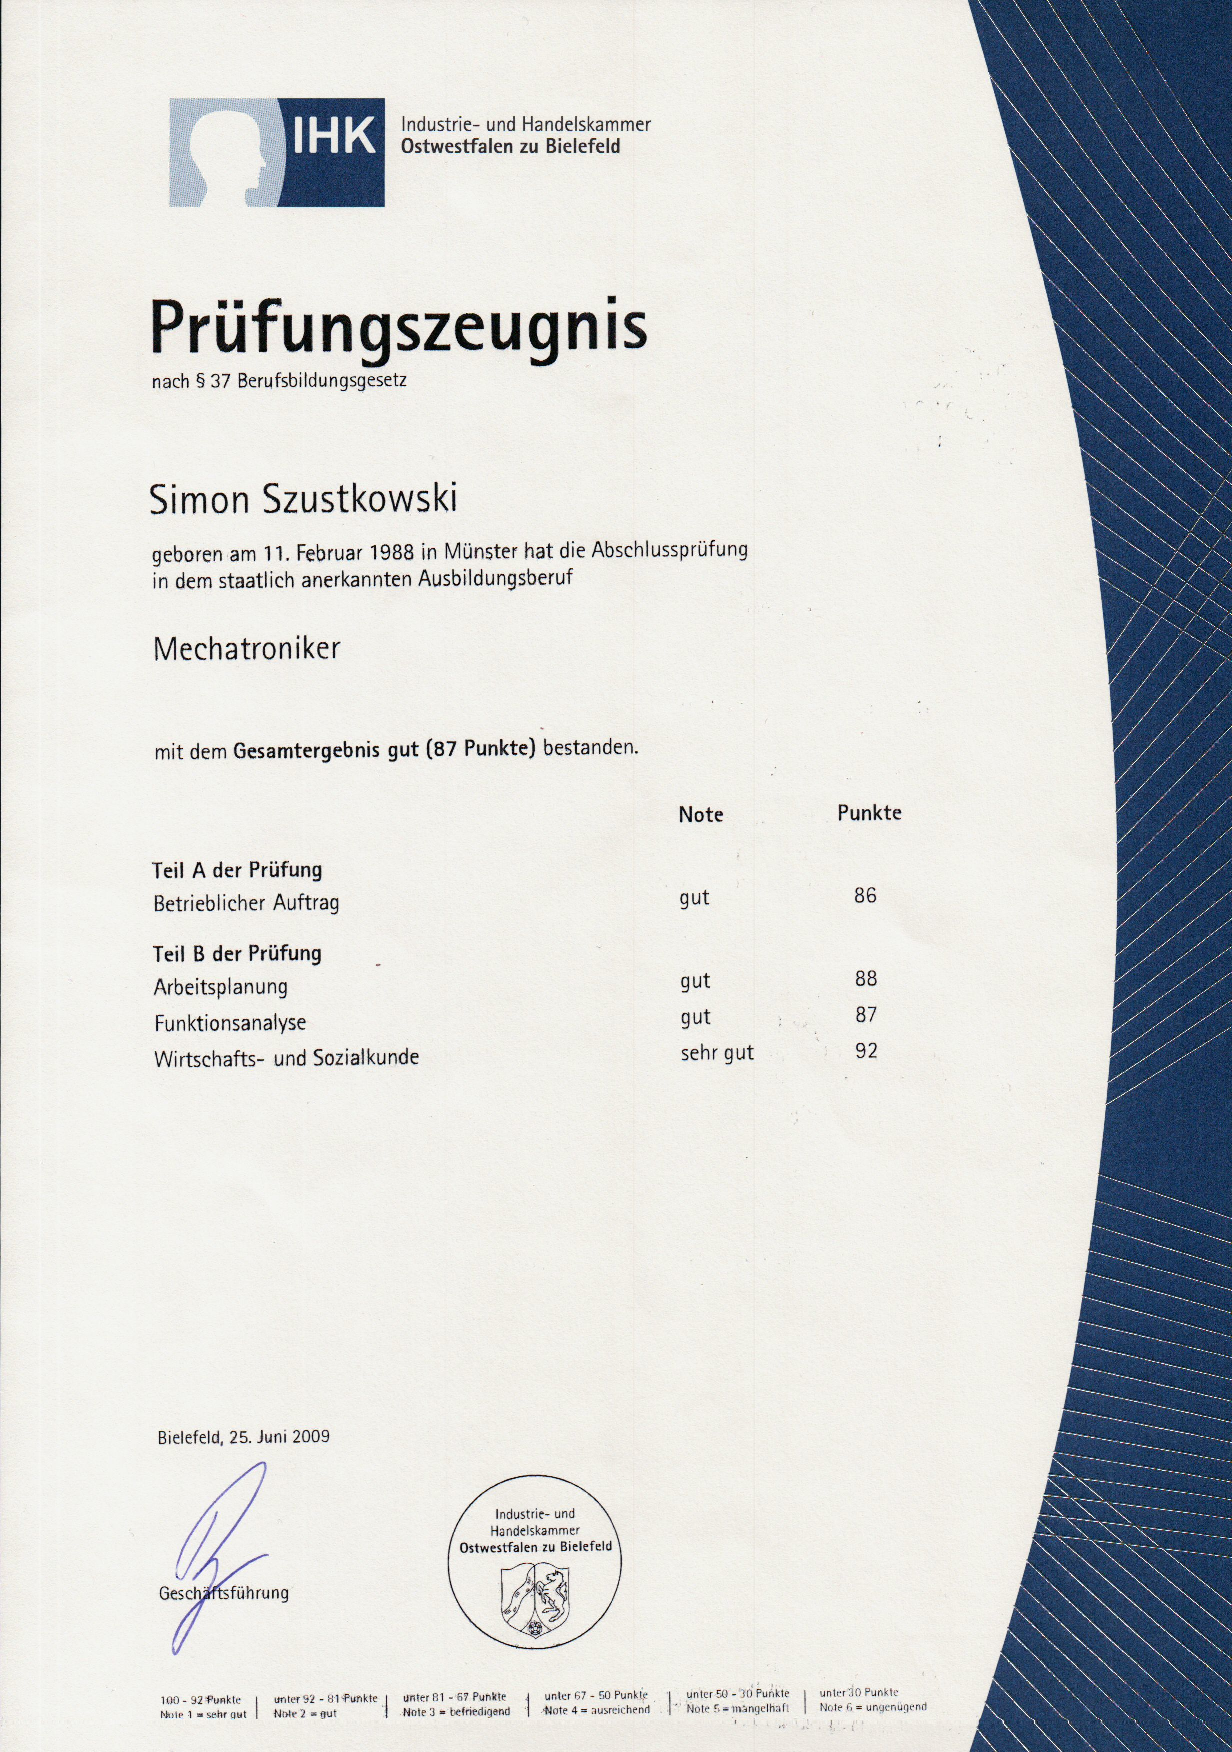
\includepdf[pages=1-]{ausbildungszeugnis.pdf}
%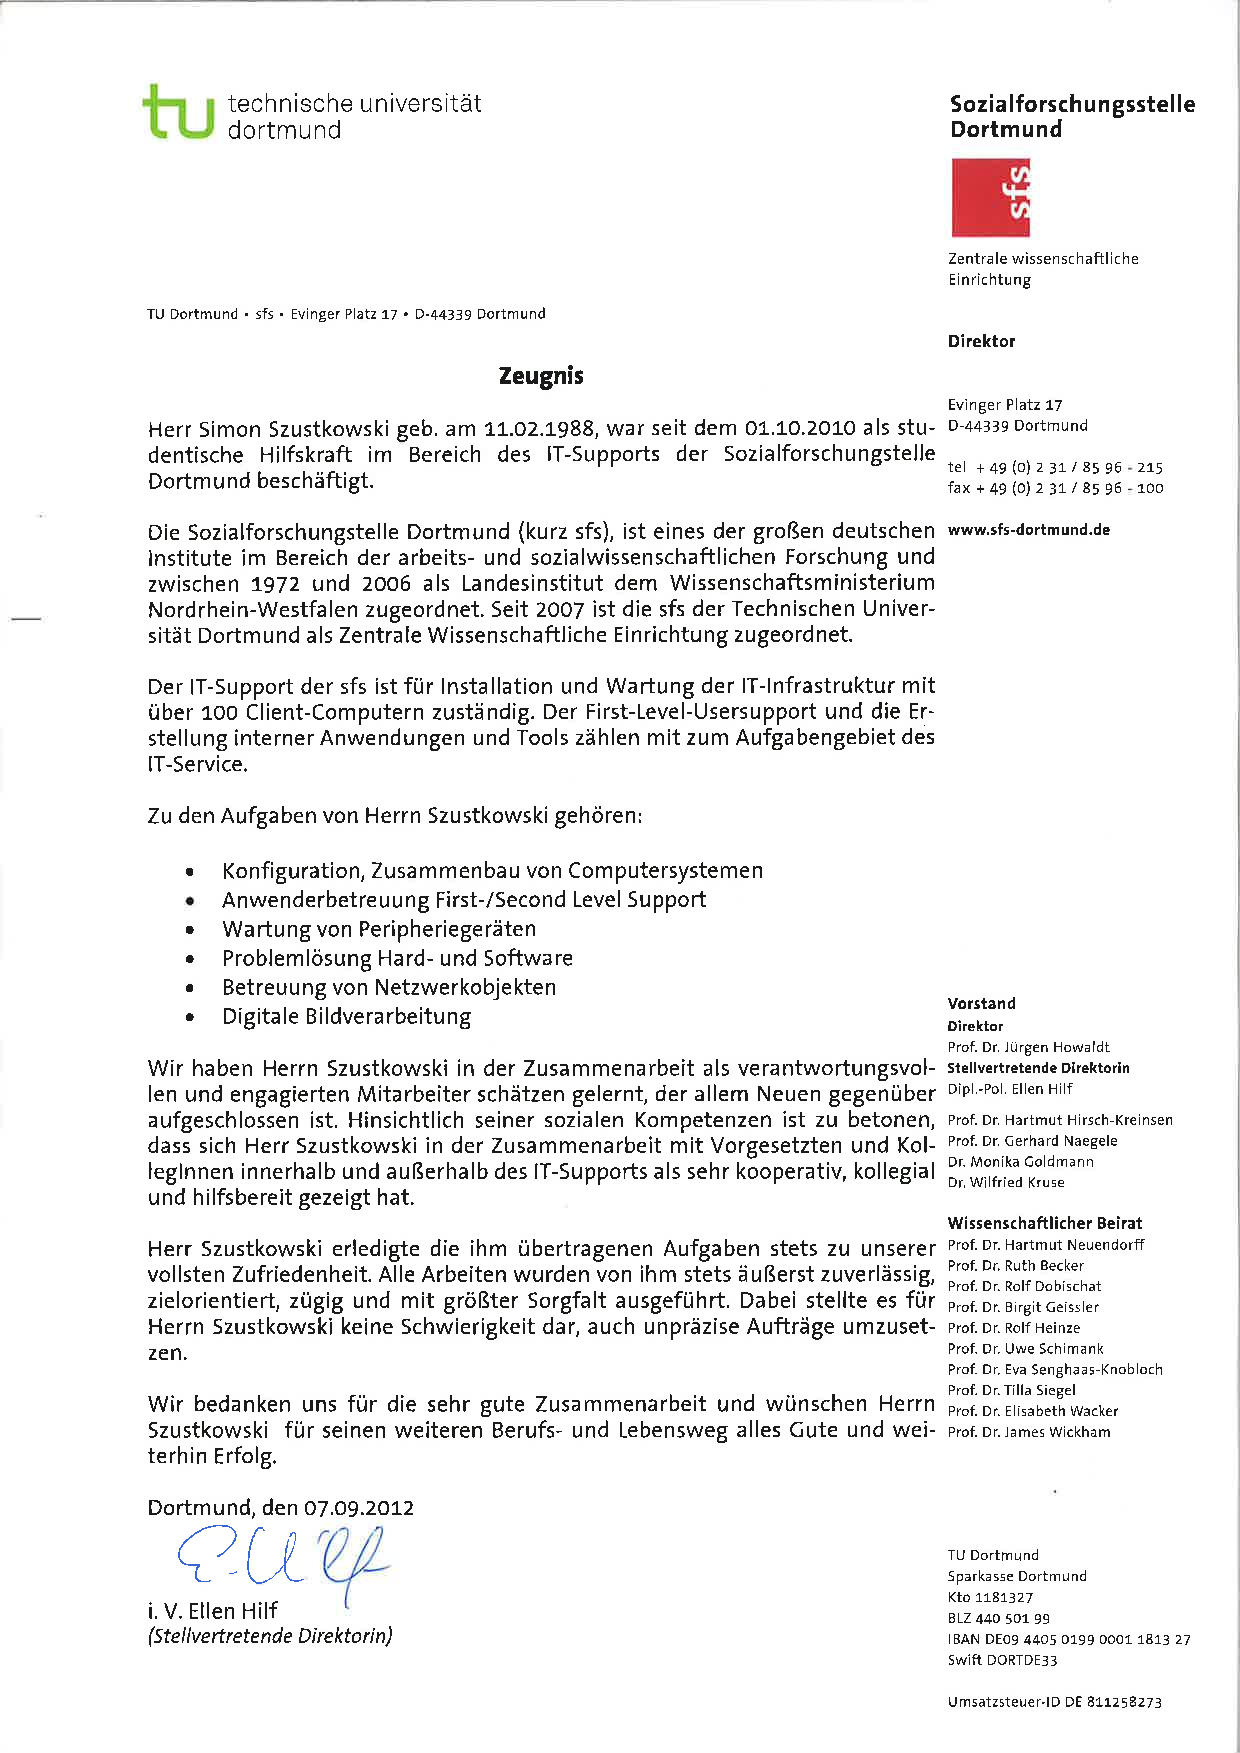
\includepdf[pages=1-]{azsfs.pdf}
%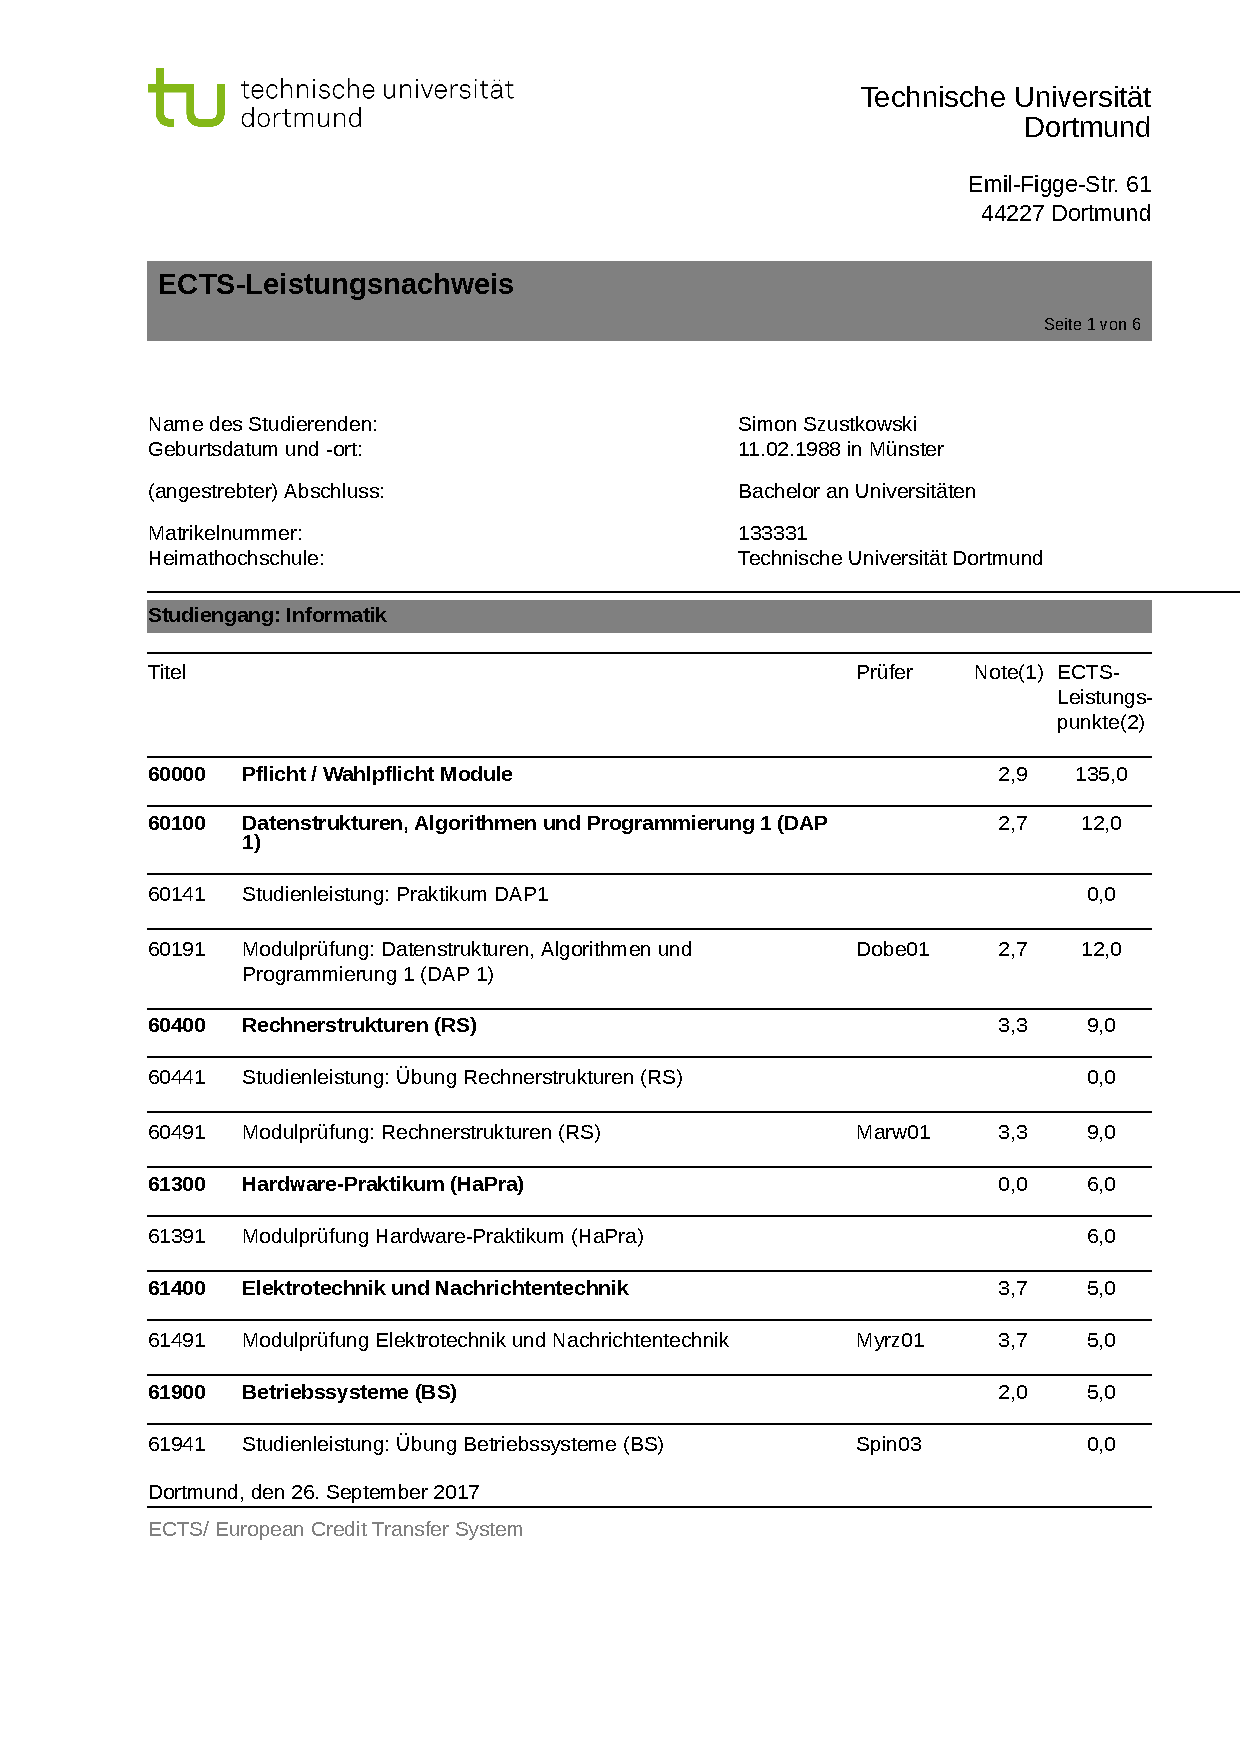
\includepdf[pages=1-]{notenspiegel.pdf}






%\chapter{Bachelor}{zeugnis}
%\vspace*{1cm}
%\begin{center}
	% \fbox{\includegraphics[height=0.85\textheight]{Bakk-Zeugnis}}	
%\end{center}

%\newpage
%\chapter{Master}{zeugnis}
%\vspace*{1cm}
%\begin{center}
	% \fbox{\includegraphics[height=0.85\textheight]{Masterzeugnis}}	
%\end{center}

%\vspace*{1cm}
%\begin{center}
	% \fbox{\includegraphics[height=0.85\textheight]{Masterzeugnis-2}}	
%\end{center}

% \newpage
% \chapter{Abschluss}{zeugnis}
% \vspace*{1cm}
% \begin{center}
% 	% \fbox{\includegraphics[height=0.85\textheight]{Abschlusszeugnis}}	
% \end{center}

\end{document}

% end of file `cv_german.tex'